\section{Preprocessing} \label{sec:preprocessing}
In this section I will describe the preprocessing steps I have applied to the dataset.

\subsection{Dataset loading} \label{sec:preprocessing-dataset-loading}
Since the dataset already have a train and a validation set, I loaded them separately and used them to train and evaluate the models.
The sets have been shuffled and the images have been resized to 256$\times$256 px.

\subsection{Normalization} \label{sec:preprocessing-normalization}
Since the image pixels are in the range [0, 255] I have normalized them to the range [0, 1] dividing each pixel by 255.
This step is important because it allows the network to converge faster and it is also important to avoid numerical issues.

\subsection{Data augmentation} \label{sec:preprocessing-data-augmentation}
The second step I have applied to the dataset is the data augmentation.
I have used the \href{https://www.tensorflow.org/api_docs/python/tf/keras/preprocessing/image/ImageDataGenerator}{ImageDataGenerator} class from TensorFlow which allows to apply different transformations to the images in real time.
So the following transformations have been applied to the images:
\begin{itemize}
    \item \textbf{Rotation}: the images have been rotated by a random angle between -20 and 20 degrees.
    \item \textbf{Width shift}: the images have been shifted horizontally by a random amount between -0.2 and 0.2 of the width.
    \item \textbf{Height shift}: the images have been shifted vertically by a random amount between -0.2 and 0.2 of the height.
    \item \textbf{Shear}: the images have been sheared by a random angle between -20 and 20 degrees.
    \item \textbf{Zoom}: the images have been zoomed by a random amount between 0 and 0.2.
    \item \textbf{Horizontal flip}: the images have been flipped horizontally with a probability of 0.5.
\end{itemize}

\begin{figure}[h]
    \centering
    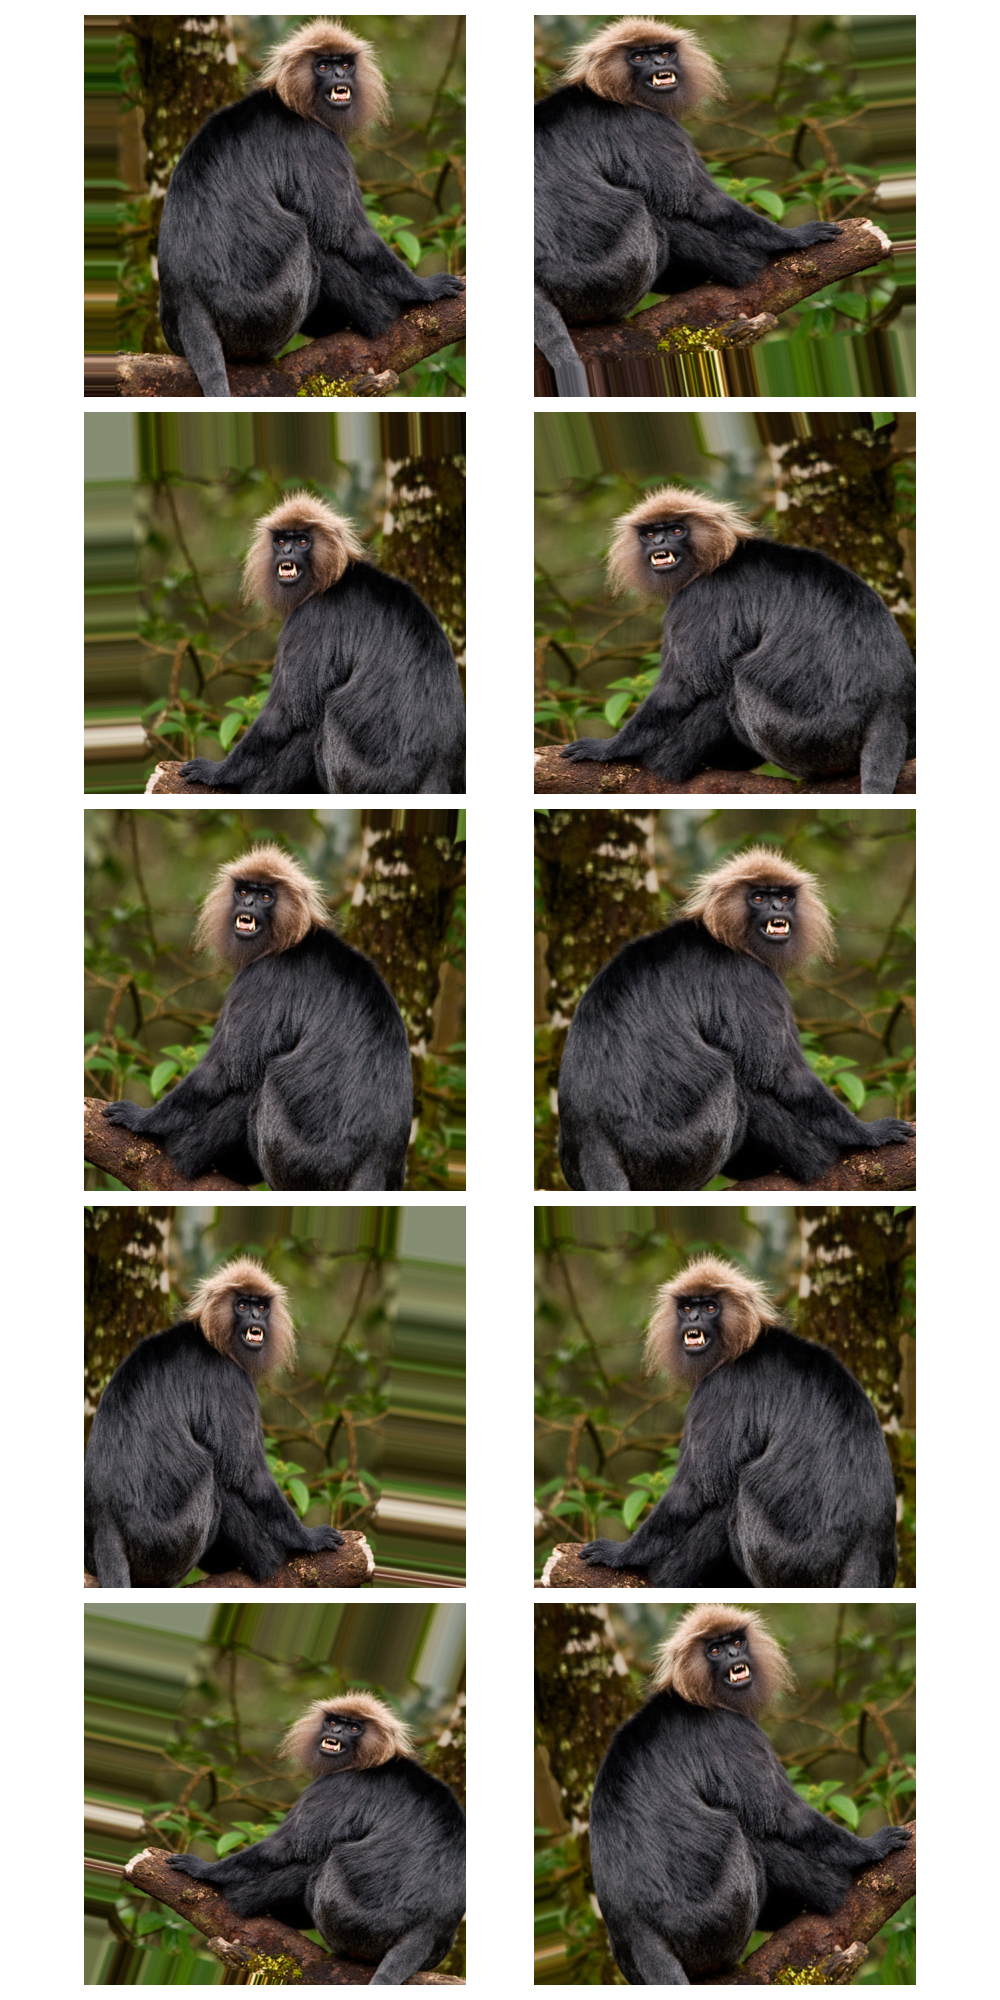
\includegraphics[height=1\linewidth]{../plot/data_augmentation.png}
    \caption{Data augmentation examples}\label{fig:data_augmentation}
\end{figure}